\documentclass[11pt,a4paper]{article}
% Encoding and language
\usepackage[utf8]{inputenc}
\usepackage[english]{babel}
% Colors
\usepackage[usenames,dvipsnames]{color}
\usepackage{colortbl}
% Paper size and margins
%\usepackage{rotating}
\usepackage{pdflscape}
%\usepackage[a4paper,showframe]{geometry}
\usepackage{vmargin}
\setmarginsrb{2cm}{2cm}{2cm}{2cm}{0cm}{0cm}{0cm}{1.5cm}
\usepackage{pdflscape}
\usepackage{afterpage}
% Indenting
\usepackage{indentfirst}
%\setlength{\parindent}{1cm}
\setlength{\parskip}{0.5cm}
% Symbols
\usepackage{amsmath}
\usepackage{amsfonts}
\usepackage{amssymb}
% Equations
\usepackage{eulervm} % upright font in eqns (Palatino)
\usepackage{cool}
\usepackage{mathtools} % for arrows
\renewcommand{\theequation}{R\arabic{equation}}
% References
\usepackage{natbib}
\bibliographystyle{apalike}
% Hyperlinks and labels
%\usepackage{showkeys}
\usepackage[linktocpage=true,plainpages=false,pdfpagelabels=false]{hyperref}
\definecolor{citecolor}{rgb}{0.2,0.7,0.9}
\definecolor{urlcolor}{rgb}{0,0,1}
\hypersetup{
    colorlinks, linkcolor={Blue},
    citecolor={Blue}, urlcolor={Black}
}
% Figures
\usepackage{subcaption}
\usepackage{alphalph}
\usepackage{tikz}
\usetikzlibrary{shapes,arrows}
\usetikzlibrary{positioning}
\usetikzlibrary{calc}
\usepackage{epstopdf}
% Tikz styles
\tikzstyle{reg} = [rounded rectangle, text width=2cm, fill=black!5, align=center, anchor=west,font=\sffamily\Large\bfseries, minimum height=1cm, inner sep=0]
\tikzstyle{rad} = [rounded rectangle, draw=none, text width=2cm, fill=red!10, align=center, anchor=west,font=\sffamily\Large\bfseries, minimum height=1cm, inner sep=0]
\tikzstyle{long} = [rounded rectangle, draw=none, text width=3.5cm, fill=black!5, align=center, anchor=west,font=\sffamily\Large\bfseries, minimum height=1cm, inner sep=0]   
\tikzstyle{add} = [scale=1.5, draw=none,fill=none,align=center]
\tikzstyle{emp} = [draw=none,fill=none]
\tikzstyle{ar} = [->,draw=black!70,line width=2]
\tikzstyle{ln} = [-,draw=black!70,line width=2]
% Title etc
\newcommand{\mytitle}{Investigation of the relationship between tropospheric ozone production efficiency and carbon bond emissions}
\newcommand{\authorname}{Maria Zamyatina}
\newcommand{\authornumber}{Student No: 100106685}
\newcommand{\degname}{Master of Science}
\newcommand{\univname}{University of East Anglia}
\newcommand{\univaddr}{University Plain \\ Norwich NR47TJ UK}
\newcommand{\depname}{School of Environmental Sciences}
\newcommand{\mydate}{\the\year}
%% Remove author and date from the maketitle command
%\makeatletter
%\renewcommand{\@maketitle}{
%\newpage
% \null
% \vskip 2em%
% \begin{center}%
%  {\LARGE \@title \par}%
% \end{center}%
% \par} \makeatother

% PDF meta-data
\hypersetup{pdftitle={\mytitle}}
\hypersetup{pdfauthor=\authorname}

\title{\mytitle}
% =========================================================================
\begin{document}

\thispagestyle{empty}
\vskip 3cm
\begin{center}
    {\Huge\bfseries\sf \mytitle \par}
    \vskip 1cm
    \sf by
    \vskip 1cm
    \large \sf \authorname \\
    \sf \authornumber
\end{center}

\begin{center}
	\large \sf Thesis presented in part-fulfilment of the degree of \degname \\ in accordance with the regulations of the \univname
\end{center}

\vskip 5cm

\begin{minipage}{0.4\textwidth}
\begin{flushleft} 
\large \sf 
\depname \\
\univname \\
\univaddr
\vskip 0.5cm
\copyright~\mydate~\authorname
\end{flushleft}
\end{minipage}

%\vskip 0.2cm

\begin{minipage}{\textwidth}
\begin{flushleft}
%\noindent
\sf This copy of the dissertation has been supplied on condition that anyone who consults it is understood to recognise that its copyright rests with the author and that no quotation from the dissertation, nor any information derived there from, may be published without the author's prior written consent. Moreover, it is supplied on the understanding that it represents an internal University document and that neither the University nor the author are responsible for the factual or interpretative correctness of the dissertation.
\end{flushleft}
\end{minipage}

\vfill

\newpage

\tableofcontents
\newpage

\begin{abstract}
Abstract.
\end{abstract}

\section{Introduction} \label{sec:intro}
The Earth’s atmosphere is the recipient of a vast range of chemical compounds emitted by natural and anthropogenic sources. The oxidation of these compounds is the main process taking place in the atmosphere that keeps their concentrations at levels that do not distort the chemical balance of the atmosphere \citep{Prinn2003}. In other words, oxidation is a removal “cleansing” mechanism for these compounds (various pollutants and greenhouse gases), and its rate is often referred to as the oxidizing capacity of the atmosphere. This capacity depends mainly on two factors: the global burden of the principal oxidants such as ozone ($O_3$), the hydroxyl radical ($OH$) and hydrogen peroxide ($H_2O_2$), and climate \citep{Prinn2003,Thompson1992}.

\subsection{Tropospheric ozone}
Tropospheric ozone ($O_3$) plays an important role in the chemical and thermal balance of the atmosphere. Although it accounts only for about 10\% of the total ozone, it is a primary precursor to the formation of hydroxyl radicals ($OH$) which in association with hydrogen peroxide ($H_2O_2$) determines the ‘cleansing’ capacity of the atmosphere \citep{Prinn2003,Tarasick2008,Thompson1992}. On the other hand, being a source of main pollutant removal agents, ozone is an air pollutant itself. Long exposure to its high concentrations causes respiratory problems in humans and damage to sensitive plant species \citep{Fowler2008}. Last but not least characteristic of tropospheric ozone is that it is an important greenhouse gas with a current estimated radiative forcing of  $0.40\pm 0.20~Wm^{–2}$ which is approximately one fifth of the $CO_2$ radiative forcing \citep{Hartmann2013,Myhre2013}. Due to these reasons a considerable interest in quantifying tropospheric ozone concentrations, budget and trends exists for more than a 100 years \citep{Becker2004}.

Unlike many other air pollutants, tropospheric ozone is not directly emitted, but produced following the oxidation of carbon monoxide ($CO$), methane ($CH_4$), and nonmethane volatile compounds (nmVOCs) in the presence of nitrogen oxides (NOx) \citep{Crutzen1973,Myhre2013}. The emissions of these precursors arise from both natural and anthropogenic sources which have intensified since pre-industrial times \citep{Parrish2014,Volz1988} (Figure \ref{fig:O3observations}). Presumably it has led to roughly a doubling in background tropospheric ozone concentration \citep{Guicherit2000,Hartmann2013,Tarasick2008,Vingarzan2004}, although contribution from another major source, transport from the stratosphere, may also took place \citep{Fowler2008}. Climate is also believed to be a key driver of ozone production and destruction since the chemical reactions affecting ozone concentration are strongly dependent on such climatic factors as temperature, rainfall and humidity. Therefore in a changing climate tropospheric ozone is not anymore a local air quality issue, but is a global pollution problem \citep{Fowler2008}.

\begin{figure}[h]
\includegraphics[width=\linewidth]{{./pics/Isaksen2009_O3}.png}
\caption{Observed surface ozone at different Northern Hemispheric surface stations \citep{Isaksen2009}.}
\label{fig:O3observations}
\end{figure}

According to the Intergovernmental Panel on Climate Change (IPCC) Fifth Assessment report (AR5) for present conditions (around year 2000) the global mean tropospheric ozone budget is approximately 331 Tg \citep{Myhre2013}. However, despite general agreement on how the drivers impact ozone concentrations at global and regional scales, its budget varies considerably between different modelling and observational studies \citep{Stevenson2006,Wild2007,Young2012}. Table \ref{tab:O3budget} demonstrates that the range of the global tropospheric ozone budget estimates is approximately 60 Tg which is 18\% of the mean. In terms of ozone production the variation is even higher and account for 28\% of the corresponding value. In that regard, two questions arise: why does the tropospheric ozone budget differ between models and observations? And secondly, why does it vary to this extent, especially in terms of production? The only way to answer these questions is to perform a rigorous investigation of the factors that drive tropospheric ozone and attribute those differences to respective factors \citep{Young2012}.

\begin{table}[h] % O3 budget
\centering
\caption{Summary of tropospheric ozone global budget model and observation estimates for present (about 2000) conditions. All uncertainties quoted as 1 standard deviation (68\% confidence interval). Adapted from \citep{Myhre2013}}
\label{tab:O3budget}
\begin{tabular}{ccl}
\hline
Burden, Tg & Production, Tg yr–1 & Reference \\
\hline
\multicolumn{3}{c}{Modelling studies} \\
$337\pm23$  & $4877\pm853$ & Young et al. (2013); ACCMIP \\
$323$	    & -	           & Archibald et al. (2011) \\
$330$	    & $4876$       & Kawase et al. (2011) \\
$312$       & $4289$       & Huijnen et al. (2010) \\
$334$       & $3826$       & Zeng et al. (2010) \\
$324$       & $4870$       & Wild and Palmer (2008) \\
$314$       & -	           & Zeng et al. (2008) \\
$319$	    & $4487$	   & Wu et al. (2007) \\
$372$	    & $5042$       & Horowitz (2006) \\
$349$	    & $4384$	   & Liao et al. (2006) \\
$344\pm39$	& $5110\pm606$ & Stevenson et al. (2006); ACCENT \\
$314\pm33$	& $4465\pm514$ & Wild (2007) (post-2000 studies) \\
\hline
\multicolumn{3}{c}{Observational studies} \\
$333$   	& -	           & Fortuin and Kelder (1998) \\
$327$	    & -	           & Logan (1999) \\
$325$	    & -	           & Ziemke et al. (2011); 60S–60N \\
$319–351$	& -	           & Osterman et al. (2008); 60S–60N \\
\hline
\end{tabular}
\end{table}

A considerable effort has been made to tackle these problems, and generally there are two possible ways of doing it. The first one implies the direct analysis of tropospheric chemical schemes used in climate-chemistry models. For example, Emmerson and Evans (2009) compared the state of the art Master Chemical Mechanism which contains approximately 5600 species and 13500 reactions \citep{Jenkin2002} with other six chemical schemes and found four significant variations between them. This approach is linked with big challenges since a modern global model is a very sophisticated representation of the climate-chemistry interactions, and therefore it is often difficult to separate influence of one reaction from another. However, even being so developed climate-chemistry models do not take into account all known chemical reactions taking place in the real troposphere. A complete representation requires many thousands of species and tens of thousands of reactions, which is beyond the numerical capabilities currently available. This significantly limits the practicable size of chemical schemes and typically involves a reduction of the number of VOCs considered and lumping the carbon from the discarded species into representative surrogates.

The second way to understanding the discrepancies between models and observations is to conduct an idealised theoretical study using a conceptual model. The advantage of this approach is that such kind of models can be quite easily constructed, and more importantly can be focused on representation of a certain chemical reactions which presumably could explain the discrepancy between models and observations. An example of such set of reactions is alkyl nitrate chemistry.

\subsection{Alkyl nitrates}
Alkyl nitrates are important tropospheric trace gases which are formed following the same chemistry that leads to the production of ozone \citep{Reeves2007}. The simplest example, in case of $CH_4$ oxidation, can be described by the set of reactions below (also shown in Figure 2).

%\documentclass[]{standalone}
\usepackage[utf8]{inputenc}
\usepackage[english]{babel}
\usepackage{amsmath}
\usepackage{amsfonts}
\usepackage{amssymb}

\usepackage{graphicx}
%\usepackage[left=2cm,right=2cm,top=2cm,bottom=2cm]{geometry}

% Figures
\usepackage{tikz}
\usetikzlibrary{shapes,arrows}
\usetikzlibrary{positioning}
\usetikzlibrary{calc}
%\usepackage{chemfig}

% Tikz styles
\tikzstyle{reg} = [rounded rectangle, text width=2cm, fill=black!5, align=center, anchor=west,font=\sffamily\Large\bfseries, minimum height=1cm, inner sep=0]
\tikzstyle{rad} = [rounded rectangle, draw=none, text width=2cm, fill=red!10, align=center, anchor=west,font=\sffamily\Large\bfseries, minimum height=1cm, inner sep=0]
\tikzstyle{long} = [rounded rectangle, draw=none, text width=3.5cm, fill=black!5, align=center, anchor=west,font=\sffamily\Large\bfseries, minimum height=1cm, inner sep=0]   
\tikzstyle{add} = [scale=1.5, draw=none,fill=none,align=center]
\tikzstyle{emp} = [draw=none,fill=none]
\tikzstyle{ar} = [->,draw=black!70,line width=2]
\tikzstyle{ln} = [-,draw=black!70,line width=2]


\begin{document}
\begin{tikzpicture}[node distance = 4cm, auto]

% Nodes: big cycle: CH4-CH302-CH3NO3-CH3O-HCHO-HO2-OH-O3
\node[reg] (ch4) {$CH_4$};
\node[add](foo1_1) at (3,-2) {};
\node[add](foo1_2) at (4,-2) {$O_2$\\$OH$};
\node[reg] (ch3o2) at (5,-4){$CH_3 O_2$};
\node[reg] (oh) at (5,4){$OH$};
\node[long] (ch3ooh) at (0,-8){$CH_3OOH$};
\node[reg] (oz1) at (0,8){$O_3$};
\node[emp] (foo2) at ($(oz1)!.5!(oh)$){};
\node[reg] (ho2) at (15,4){$HO_2$};
\node[add] (oz_up) at ($(ho2)!.5!(oh) + (0,0.5)$){$O_3$};
\node[reg] (h2o2) at (17.5,7.5){$H_2O_2$};
\node[add] (ho2_) at (16.5,6){$HO_2$};
\node[emp] (nox_top) at ($(ho2)!.5!(oh) + (0,1.5)$){};
\node[reg] (ch3o) at (15,-4){$CH_3 O$};
\node[reg] (hcho) at (20,0){$HCHO$};
\node[emp] (foo5) at (19,-2){};
\node[long] (ch3no3) at (10,-10){$CH_3 NO_3$};
\node[add] (foo1_2) at (7,-9) {$NO$};
%\node[emp] (dep1) at (11,-12){};
%\node[add] (dep1_) at (10.3,-11.3){deposition};

%Nodes: Bottom NOx cycle + misc
\node[add] (no_1) at (7,-6){$NO$};
\node[add] (no2_1) at (13,-6){$NO_2$};
\node[emp] (nox_bottom) at ($(no_1)!.5!(no2_1)+(0,2)$){};
\node[emp] (foo7) at (11.5,-7.5){};
\node[add] (hv_11) at (12,-7){$h\nu$};
\node[reg] (o3_1) at (9.25,-8.75){$O_3$};
\node[add] (o2_1) at (11.2,-7.9){$O_2$};
\node[emp] (foo3) at (16,-8){};
\node[add] (hv_12) at (15,-8.75){$h\nu$};
\node[emp] (foo4) at (19,-8){};
\node[add] (oh_) at (20,-6.5){$OH$};
\node[add] (o2_) at (18,-3){$O_2$};

%Nodes: Top NOx cycle + misc
\node[add] (no2_2) at ($(ho2)!.5!(oh)+(-3,3.5)$){$NO_2$};
\node[add] (no_2) at ($(ho2)!.5!(oh)+(3,3.5)$){$NO$};
\node[add] (hv_2) at (10,9){$h\nu$};
\node[reg] (o3_2) at (13,10.5){$O_3$};
\node[add] (o2_2) at (12.75,9.75){$O_2$};
\node[emp] (foo6) at (11.5,9.5){};

%Nodes: CO & CO2
\node[reg] (co) at ($(ho2)!.5!(oh)+(-4,-3)$){$CO$};
\node[reg] (co2) at ($(ho2)!.5!(oh)+(2,-3)$){$CO_2$};
\node[emp] (cc_o2) at ($(ho2)!.5!(oh)+(0,-2.5)$){};
\node[emp] (cc_1) at ($(ho2)!.5!(oh)+(-0.5,-1.5)$){};
\node[emp] (cc_2) at ($(ho2)!.5!(oh)+(0.5,-1.5)$){};
\node[add] (cc_o2) at ($(ho2)!.5!(oh)+(0,-2)$){$O_2$};

%Nodes: HCHO decompostion
\node[long] (co_2ho2) at (25,3){$CO~+~2HO_2$};
\node[add] (hcho_hv1) at ($(hcho)!.5!(co_2ho2)$){$h\nu$};
\node[long] (co_h2) at (25,0){$CO~+~H_2$};
\node[add] (hcho_hv2) at ($(hcho)!.5!(co_h2)+(0.25,0.25)$){$h\nu$};
\node[long] (co_ho2) at (25,-3){$CO~+~HO_2$};
\node[add] (hcho_oh) at ($(hcho)!.5!(co_ho2)+(0.25,0)$){$OH$};
%\node[long] (hno3dep) at (25,-6){\small $CO~+~HO_2~+~HNO_3$\\ deposition?};
%\node[add] (hcho_no3) at ($(hcho)!.5!(hno3dep)$){$NO_3$};

%Nodes: after decomposition HO_2 + CO_2
\node[emp] (decomp) at ($(co_2ho2)!.5!(co_ho2)+(3,0)$){};
\node[long] (decomp2) at ($(decomp)+(2,0)$){$HO_2~+~CO_2$};
\node[add] (decomp_oh) at ($(decomp)+(1,0.5)$){$OH$};

% Connections: big cycle
\draw[ln] (oh.west) to [out=180,in=90](foo1_1.center);
\draw[ln] (ch4.east) to [out=0,in=90](foo1_1.center);
\draw[ar] (foo1_1.center) to [out=270,in=180](ch3o2.west);
\draw[ar] (ch3o2) to (ch3ooh);
\node[add](foo1) at ($(ch3o2)!.5!(ch3ooh) + (-1,0)$) {$HO_2$};
%\draw[ar] (oz1) to node[right]{$h\nu$}(foo2.north west);
\draw[ar] (oz1) to (oh);
\node[add] (o3_to_OH) at ($(oz1)!.5!(oh) + (0.5,0.5)$){$h\nu$\\ $H_2O$};
%\draw[ar] (foo2.south east) to node[right]{$H_2O$}(oh);
\draw[ar] (ho2) to (h2o2);
\draw[ln] (ho2.north west) to [out=135,in=0](nox_top.center);
\draw[ar] (nox_top.center) to [out=180,in=45](oh.north east);
\draw[ar] (ho2) to (oh);
\draw[ln] (ch3o2) to (nox_bottom.center);
\draw[ar] (nox_bottom.center) to (ch3o);
\draw[ar] (ch3o2.south) to [out=270,in=180](ch3no3.west);
\draw[ln] (ch3o.east) to [out=0,in=270](foo5.center);
\draw[ar] (foo5.center) to [out=90,in=0](ho2.east);
\draw[ar] (foo5.center) to [out=90,in=180](hcho.west);

% Connections: bottom NOx cycle + misc
\draw[ln] (no_1.north) to [out=90,in=180](nox_bottom.center);
\draw[ar] (nox_bottom.center) to [out=0,in=90](no2_1.north);
\draw[ln] (no2_1.south) to [out=270,in=0](foo7.center);
\draw[ar] (foo7.center) to [out=180,in=90](o3_1.north);
\draw[ar] (foo7.center) to [out=180,in=270](no_1.south);
\draw[ln] (ch3no3.east) to [out=0,in=270](foo3.center);
\draw[ar] (foo3.center) to [out=90,in=270](ch3o.south);
\draw[ar] (foo3.center) to [out=90,in=0](no2_1.east);
\draw[ln] (ch3no3.east) to [out=0,in=270](foo4.center);
\draw[ar] (foo4.center) to [out=90,in=270](hcho.south);
\draw[ar] (foo4.center) to [out=90,in=0](no2_1.east);
%\draw[ar] (ch3no3.south) -- (dep1.center);

% Connections: top NOx cycle
\draw[ln] (no_2.south) to [out=270,in=0](nox_top.center);
\draw[ar] (nox_top.center) to [out=180,in=270](no2_2.south);
\draw[ln] (no2_2.north) to [out=90,in=180](foo6.center);
\draw[ar] (foo6.center) to [out=0,in=90](no_2.north);
\draw[ar] (foo6.center) to [out=0,in=270](o3_2.south);

%Connections: CO & CO2
\draw[ln] (oh.south east) to [out=315,in=180](cc_1.center);
\draw[ln] (co.north east) to [out=45,in=180](cc_1.center);
\draw[ln] (cc_1.center) to [out=0,in=180](cc_2.center);
\draw[ar] (cc_2.center) to [out=0,in=225](ho2.south west);
\draw[ar] (cc_2.center) to [out=0,in=135](co2.north west);

%Connections: HCHO decomp
\draw[ar] (hcho.east) to [out=0,in=180](co_2ho2.west);
\draw[ar] (hcho.east) to [out=0,in=180](co_h2.west);
\draw[ar] (hcho.east) to [out=0,in=180](co_ho2.west);
%\draw[ar] (hcho.east) to [out=0,in=180](hno3dep.west);

\draw[ln] (co_2ho2.east) to [out=0,in=180](decomp.center);
\draw[ln] (co_h2.east) to [out=0,in=180](decomp.center);
\draw[ln] (co_ho2.east) to [out=0,in=180](decomp.center);
\draw[ar] (decomp.center) to [out=0,in=180](decomp2.west);


\end{tikzpicture}

\end{document}

In the presence of UV light shorter than 320 nm and water vapour $O_3$ photolysis is the main source of OH radicals in the troposphere:
\begin{equation} \label{eq:O3hv}
O_3 + hv \rightarrow O(^1D) + O_2
\end{equation}
\begin{equation} \label{eq:O1D+H2O}
O(^1D) + H_2O \rightarrow 2OH
\end{equation}
Once formed the OH radicals react mainly with $CO$ and $CH_4$ to initiate the $O_3$ formation or removal cycles by producing peroxy radicals ($HO_2$, $CH_3O_2$):
\begin{equation} \label{eq:OH+CO}
OH + CO \rightarrow HO_2 + CO_2
\end{equation}
\begin{equation} \label{eq:OH+CH4}
OH + CH_4 \rightarrow CH_3O_2 + H_2O
\end{equation}

The fate of the peroxy radicals depends on the presence of NOx. At low NOx levels (remote regions), the $HO_2$ radical reacts with another HO2 to form hydrogen peroxide, H2O2, or with the methyl peroxy radical, $CH_3O_2$, to form methyl hydrogen peroxide ($CH_3OOH$):
\begin{equation} \label{eq:HO2+HO2}
HO_2 + HO_2 \rightarrow H_2O_2 + O_2
\end{equation}
\begin{equation} \label{eq:HO2+CH3O2}
HO_2 + CH_3O_2 \rightarrow CH_3OOH + O_2
\end{equation}
On a whole, at low NOx levels a net $O_3$ loss takes place, because the reaction sequence is initiated by $O_3$ photolysis. Plus under the same conditions, some additional $O_3$ removal occurs due to the re-action of $HO_2$ radicals with $O_3$,
\begin{equation} \label{eq:HO2+O3}
HO_2 + O_3 \rightarrow OH + 2O_2
\end{equation}
leading to the regeneration of OH radicals as part of an $O_3$ depleting HOx catalytic cycle.

At intermediate NOx levels (rural areas of most industrialised countries), the peroxy radicals react with nitrogen monoxide ($NO$) to form nitrogen dioxide ($NO_2$) with the subsequent photolysis of $NO_2$ generating $O_3$:
\begin{equation} \label{eq:HO2+NO}
HO_2 + NO \rightarrow NO_2 + OH
\end{equation}
\begin{equation} \label{eq:CH_3O_2+NO}
CH_3O_2 + NO \rightarrow NO_2 + CH_3O
\end{equation}
\begin{equation} \label{eq:NO2hv}
NO_2 + hv \rightarrow NO + O(^3P)
\end{equation}
\begin{equation} \label{eq:O3P+O2}
O(^3P) + O_2 + M \rightarrow O_3 + M
\end{equation}
As it is shown in Figure 2 reactions (8) and (9) form part of the free-radical propagated $O_3$ forming cycles, which may occur a number of times before being halted by a radical termination reactions (not shown). However, the reaction of $CH_3O_2$ with NO is a two-channel reaction \citep{Day2003}, and its second branch can terminate the $O_3$ forming cycle earlier by producing an alkyl nitrate, in this case methyl nitrate ($CH_3ONO_2$):
\begin{equation} \label{eq:CH3NO3form}
CH_3O_2 + NO \rightarrow CH_3ONO_2
\end{equation}

Being a reservoir for the short lived NOx and having atmospheric lifetimes ranging from several days to about a month \citep{Reeves2007} alkyl nitrates can be transported over long distances, and then lost through photolysis and reaction with $OH$:
\begin{equation} \label{eq:CH3NO3hv}
CH_3ONO_2 + hv \rightarrow CH_3O + NO_2
\end{equation}
\begin{equation} \label{eq:CH3NO3+OH}
CH_3ONO_2 + OH \rightarrow HCHO + NO_2
\end{equation}
It means that alkyl nitrates can ‘release’ $NO_2$ back to the atmosphere after a while, and in association with reactions (10) and (11) start a new $O_3$ formation cycle being quite away from the source.

The free-radical propagated oxidation of hydrocarbons leads to the generation of carbonyl compounds, in this case formaldehyde ($HCHO$). Its further oxidation and photolysis contributes to radical generation:
\begin{equation} \label{eq:HCHOhv1}
HCHO + hv \rightarrow 2HO_2 + CO
\end{equation}
\begin{equation} \label{eq:HCHOhv2}
HCHO + hv \rightarrow CO + H_2
\end{equation}
\begin{equation} \label{eq:HCHO+OH}
HCHO + OH \rightarrow HO_2 + CO
\end{equation}
As a result, the formation of $HCHO$ has an impact on the rates of the oxidation cycles described above, through secondary radical generation \citep{Fowler2008}.
At high NOx levels (urban environment) reactions (8) and (9) dominate for $CH_3O_2$ and $HO_2$, but $O_3$ formation becomes inhibited by further increases in NOx. In other words, at high NOx regime the $O_3$ formation rate becomes sensitive to the concentration of $CH_4$ or $CO$ and to inputs of other VOCs \citep{Fowler2008}.

To sum up, alkyl nitrates are produced as a minor branch of the reaction of peroxy radicals with NO \citep{Day2003}. Since these compounds are removed from the troposphere by photolysis and OH oxidation they can provide information on photochemical evolution of an air mass through relationships with their parent hydrocarbons \citep{Bertman1995}. Acting as reservoir species for reactive nitrogen (NOy) and having a relatively long atmospheric lifetimes alkyl nitrates play an important role in long range transport of NOx. Furthermore, alkyl nitrates link to ozone and carbonyl production making them useful tracers for both species \citep{Worton2010}. Despite their relative importance alkyl nitrates are usually not included in the climate-chemistry models, for example in UKCA (Reeves, personal communication), which potentially could lead to discrepancies between models and observations described before. 

!! from \citep{Finlayson-Pitts2000}
The relationship between the peroxy radical concentration and the ozone photolysis rate constant for these higher NO conditions can be again approximated using steady-state analysis [..]. While OH is recycled in its reactions with CO and CH4 via HO2, it is pernanetly removed at higher NOx concentrations by the reaction of OH with NO2, forming nitric acid:
OH + NO2 = M = HONO2 (113).
This reaction is primarily a daytime reaction because most OH sources are photolytic in nature. As a result, the NO2 reaction with OH competes!!!! with NO2 photolysis (page 290/993)!!
         Rate coeff (OH+NO2 = HNO3)  J(NO2 = NO+O)
Book     2.47e-30          7.00e-3
My model 1.15e-11          4.39e-03
Thus, the reaction with OH is not usually a dominant loss process for NO2, but it is still sufficiently fact to from significant amounts of HNO3 during the day, particularly in polluted regions with relatively large NO2 concentrations.
Nitric acid undergoes both wet and dry deposition rapidly and can be neutralized by ammonia, the major gaseous base found in the atmosphere.

\subsection{Motivation}
lalalaep

\section{Overall objective and specific aims}
\subsection{Overall objective}
The overall purpose of this research is to investigate the impact of alkyl nitrate chemistry on ozone production efficiency.
\subsection{Specific aims}
Specific aims are:
\begin{itemize}
\item to investigate of the relationship between ozone production and carbon bond emissions (see Data and Methods);
\item to analyse the impact of inclusion of alkyl nitrates chemistry on this relationship;
\item to analyse everything mentioned above in various NOx regimes.
\end{itemize}

\section{Literature review} \label{sec:data}
Alkyl nitrates ($RONO_2$) are organic tropospheric trace gases. They are produced photochemically through the oxidation of their parent hydrocarbons \citep{Roberts1990} or emitted directly from equatorial oceans \citep{Blake2003} and biomass burning \citep{Simpson2002}. Being involved in the ozone production chemistry, these species can act as reservoirs of nitrogen oxides which availability largely affects the production of ozone \citep{Reeves2007}. Since the alkyl nitrates have atmospheric lifetimes ranging from several days to about a month, they can redistribute nitrogen oxides presented over polluted continental regions to clean remote marine environments, and therefore are considered as one of the tracers for determining the anthropogenic influence \citep{Atherton1989, Reeves2007, Worton2005}.

Alkyl nitrates are removed from the atmosphere by photolysis \citep{Turberg1990} or through oxidation by hydroxyl radical ($OH$) \citep{Talukdar1997}. Photolysis is the dominant loss mechanism for the compounds with short carbon chains and becomes more important with decreasing carbon number. Reaction with $OH$ follows the opposite trend and is most important for the pentyl nitrates and higher.

Owing to the existence of the relationship between alkyl nitrates and their parent hydrocarbons, measurements of their concentrations can provide information on the extent of photochemical processing in the air mass. \cite{Bertman1995} developed a kinetic approach to describe this relationship through the evolution of the ratio of alkyl nitrate to its parent hydrocarbon as a function of time. This approach has been extensively used to study air mass photochemical ageing at several sites, in North America \citep{Bertman1995, Roberts1998}, China \citep{Simpson2006}, the British Isles \citep{Worton2010} and over the Pacific \citep{Simpson2003} and North Atlantic Ocean \citep{Reeves2007}.

\cite{Bertman1995} found that the theoretical ratios of  2-butyl nitrate to n-butane and 2- and 3-pentyl nitrates to pentane strongly agree with those measured from the ambient air showing no evidence for primary sources of these nitrates. On the contrary, measurements of the other ratios, ethyl/ethane, n-propyl nitrate/propane, and 2-propyl nitrate/propane, appeared to be significantly higher than predicted, relative to the 2-butyl nitrate/n-butane ratio, meaning that there should be an additional source of these alkyl nitrates. \cite{Roberts1998} generally approved the theory by comparing Bertman's conclusions with the results from a new observational dataset.

Using methyl nitrate as a tracer of marine $RONO_2$ \cite{Simpson2006} revealed that the South China Sea in not a region of strong $RONO_2$ emissions suggesting that photochemical rather marine production of alkyl nitrates is dominant at the site.

\cite{Worton2010} found that the photochemical source of the short-chain alkyl nitrates originates mostly from the photochemical oxidation and decomposition of longer-chain compounds rather than from the oxidation of the parent hydrocarbons as it is thought in the previous studies.

The brief description of the measurement sites and data is presented in section \ref{sec:data}. In section \ref{sec:method} the methodology used in this work is defined. Section \ref{sec:res} contains the results. Section \ref{sec:discuss} discusses the results, particularly focusing attention on the analysis of the discrepancy between the observational data and the results of theoretical modelling. Conclusions constitute section \ref{sec:conclusion}.

! Since the most alkoxy radicals ($RO$) react rapidly with $O_2$ under atmospheric conditions and most large (>=C4) alkoxy radicals also rapidly decompose or isomerize, alkyl nitrate formation from reaction RO+NO2 = RONO2 is relatively unimportant for most organics under atmospheric conditions while observations showed that the reaction RO2+NO = RONO2 gives a higher yield (from \citep{Atkinson2000}, actually from 1982).

! Since one of the main mechanisms of the alkyl nitrate production (>C3!!) is the gas gas phase oxidation of alkanes by OH in the presence of NOx (\citep{Newland2013}).

\subsection{Bertman}
Below is the simplified scheme of atmospheric hydrocarbon oxidation leading to the formation of alkyl nitrates (see also Fig. \ref{fig:scheme_bertman}). It begins from the process of $H$ abstraction by the $OH$ radical where the fraction of the primary or secondary radical is denoted by $\alpha_1$.
\begin{equation} \label{eq:alkane_oh}
RH + \bullet OH \xrightarrow{k_1, \alpha_1} R\bullet + H_2O
\end{equation}
The resulting radical rapidly reacts with $O_2$ and forms an alkyl peroxy radical ($R\bullet$):
\begin{equation} \label{eq:rad_o2}
R\bullet + O_2 \xrightarrow{k_2} ROO\bullet
\end{equation}
Then the alkyl peroxy radical reacts with $NO$, when it can either lose an oxygen atom to form alkoxy radical ($RO\bullet$) or bond with $NO$ to form an alkyl nitrate. The former reaction is a crucial in the net production of tropospheric ozone, since photolysis of $NO_2$ is the main photochemical source of $O_3$ in the troposphere.
\begin{subequations} \label{eq:peroxy_no0}
\begin{align}
ROO\bullet + NO &\xrightarrow{k_3, (1-\alpha_3)} RO\bullet + NO_2 \label{eq:peroxy_no1}\\
ROO\bullet + NO &\xrightarrow{k_3, \alpha_3} RONO_2 \label{eq:peroxy_no2}
\end{align}
\end{subequations}
In other words, a branching ratio $\alpha_3$ of the reactions between alkyl peroxy radicals and $NO$ leads to formation of nitrate products via rearrangement of a high-energy intermediate \citep{Bertman1995}. The branching ratio $\alpha_3$ is larger when the parent alkane is larger and is a function of temperature and pressure.

\begin{figure}[h]
\centering
\begin{tikzpicture}[node distance = 4cm, auto]
\node[reg] (rh) {$RH$};
\node[rad] (roo) at (4,0){$ROO\bullet$};
\node[add] (oh) at (3,0.3) {$\bullet OH$};
\node[rad] (roor) at (4,-2){$ROOR'$};
\node[add] (r_oo) at (3.7,-1) {$R'OO\bullet$};
\node[reg] (rono2) at (2,3){$RONO_2$};
\node[rad] (ro) at (6,3){$RO\bullet$};
\node[add] (alpha) at ($(roo)!.5!(rono2) + (-1,-0.2)$) {$\alpha_3$};
\node[add] (alpha2) at ($(roo)!.5!(ro) + (1,-0.2)$) {$1-\alpha_3$};
\node[add] (no) at ($(roo)+(0,1.5)$) {$NO$};
\node[reg] (rcho) at (9,3){$RCHO$};
\node[add] (prod) at (0,3){\textit{products}};

\draw[ar] (rh.east) to [out=0,in=180](roo.west);
\draw[ar] (roo.south) to [out=270,in=90](roor.north);
\draw[ar] (roo.north) to [out=90,in=270](rono2.south);
\draw[ar] (roo.north) to [out=90,in=270](ro.south);
\draw[ar] (rono2.west) to [out=180,in=0](prod.east);
\draw[ar] (ro.east) to [out=0,in=180](rcho.west);
\end{tikzpicture}
\caption{Schematic representation of the alkyl nitrate chemistry and their formation through the photooxydation of alkanes. Adapted from \citep{Bertman1995}.}
\label{fig:scheme_bertman}
\end{figure}

Apart from $NO$, alkyl peroxy radicals can react with each other and give peroxides, without formation of nitrates. As the eqs. \eqref{eq:peroxy_no0} outline, whether $ROO\bullet$ will bond with nitrates or with other peroxy radicals depends partially on $NO$ concentration. The reaction between $ROO\bullet$ and $NO$ is more likely when nitrate concentration is high.

The alkyl nitrates are removed from the atmosphere through photolysis and reaction with hydroxyl radical.
\begin{equation} \label{eq:an_photo}
RONO_2 + h\nu \xrightarrow{j_4} RO\bullet + NO_2
\end{equation}
\begin{equation} \label{eq:an_oh}
RONO_2 + OH \xrightarrow{k_5} \mathit{products}
\end{equation}
The relative importance of these two loss reactions depends generally on the net UV intensity and the size of the carbon chain in alkyl nitrates. Photolysis is relatively more important for nitrates with $< C_4$, while nitrates with longer chains ($\geq C_5$) tend to react faster with $OH$. In case of butyl nitrates both mechanisms are of similar significance \citep{Worton2010}.

Assuming that the only source of alkyl nitrates is the $OH$ reaction with alkane, and that reactions take place in $NO$-rich atmosphere (so no $ROO\bullet$ self-reactions occur), the alkyl nitrate part in this generalised scheme can be reduced to the two equations of formation and loss:
\begin{subequations} \label{eq:an_form_loss0}
\begin{align}
RH &\xrightarrow{\beta k_A} RONO2 \label{eq:an_form_loss1}\\
RONO_2 &\xrightarrow{k_B} \mathit{products} \label{eq:an_form_loss2}
\end{align}
\end{subequations}
where $k_A = k_1[OH]$ and $k_B=j_4 + k_5[OH]$. The factor $\beta=\alpha_1\alpha_3$ takes into account the fraction of $H$ atom abstraction from the particular hydrocarbon (with the reaction rate $k_1$) and the branching ratios leading to the nitrate. The photolytic loss rate of $RONO_2$ is denoted by $j_4$, and $k_5$ is the rate of alkyl nitrate destruction by $OH$.

These kinetic equations lead to the ordinary differential equations which can be integrated in time ($t$) giving a relationship between the alkyl nitrates and their parent alkanes concentrations:
\begin{equation} \label{eq:integral}
\frac{[RONO_2]}{[RH]} = \frac{\beta k_A}{k_B - k_A}\left(1-e^{(k_A - k_B)t}\right)+\frac{[RONO_2]_0}{[RH]_0}e^{(k_A - k_B)t}
\end{equation}
where subscript $0$ denotes the initial concentrations.

A further good approximation is that there is no alkyl nitrate initially (\textit{i.e.} no direct emissions), hence, the second term in eq. (\eqref{eq:integral}) becomes zero. Finally, the evolution of alkyl nitrates in an air mass can be modelled using the following formula.
\begin{equation} \label{eq:model}
\frac{[RONO_2]}{[RH]} = \frac{\beta k_A}{k_B - k_A}\left(1-e^{(k_A - k_B)t}\right)
\end{equation}
It has to be noted that eq. \eqref{eq:model} assumes no mixing with surrounding air. This simplification is reasonable only when mixing affects both the parent alkane and the corresponding alkyl nitrate similarly, keeping the ratios in eqs. \eqref{eq:integral} and \eqref{eq:model} the same \citep{Reeves2007}.

\section{Methodology} \label{sec:method}
\subsection{Model development and description}
A zero-dimensional (box) model is developed to investigate the impact of alkyl nitrate chemistry on ozone production efficiency. Its code is written using FACSIMILE for Windows. FACSIMILE is a special high-level programming language which is a powerful modelling tool designed to efficiently solve differential equations including those resulting from a set of chemical reactions.

! \citep{Newland2013}
[The model is written using the programming language FACSIMILE (Curtis and Sweetenham, 1987) and the differential equations are assembled and integrated using the Gear’s method (1971). The mixing ratios of the input species in the model are driven entirely by the emissions, the loss processes and the transport with no redistribution of the burden to ensure that mixing ratios agree with observations.]

The model is intended to represent the steady state of the troposphere under mean summer daytime meteorology and clear skies. To achieve that a number of assumptions have been made. First, the model assumes a uniform mixing of individual constituents of the troposphere, second, there are no atmospheric transport (no 'winds') and no emissions of species into the box meaning that the time evolution of each species is controlled by the chemical interactions alone and determined by their initial concentrations. The air temperature and relative humidity are assumed to be $25^{\circ}C$ and 70\% respectively and are fixed in all model runs. Other assumptions concerning the chemical mechanism and photolysis rates can be found in the following sections.

\subsection{Chemical mechanism}
The chemical mechanism of the model is based on recommendations from \citep{Atkinson2004} and information from the Master Chemical Mechanism, MCM v3.3 \citep{Jenkin1997,Saunders2003}, retrieved via website: http://mcm.leeds.ac.uk/MCM. On a whole it includes 90 species and 165 reactions. The mechanism is developed to represent the chemistry that governs the production and loss of ozone, hydrocarbons and alkyl nitrates. These include:

! \citep{Newland2013}
[The majority of the kinetic reaction rates and photochemical data used in the full chemistry model were taken from the IUPAC Subcommittee for Gas Kinetic Data Evaluation (http://www.iupac-kinetic.ch.cam.ac.uk; Atkinson et al., 2004; Atkinson et al., 2006; Atkinson et al., 2008). If the required data were not provided by IUPAC then data were taken from the NASA / JPL ‘Chemical Kinetics and Photochemical Data for Use in Atmospheric Studies: Evaluation No. 17’ (Sander et al., 2011). Both these sources consider the full range of literature available on each reaction and provide a recommendation based on a synthesis of this data. There are sometimes minor differences between the recommendations of each organisation.]

\begin{itemize}
\item the formation of ozone as a result of the photolysis of $NO_2$ followed by the reaction of ground-state oxygen atom ($O(^3P)$) with molecular oxygen and a third body, M ($N_2$ or $O_2$);
\item the loss of ozone through its photolysis and reactions with $O(^3P)$, $OH$, $HO_2$ and $NO$, among which the last is of particular interest because it gives back $NO_2$;
\item the formation of alkylperoxy radicals ($RO_2$) from oxidation of the hydrocarbons;
\item the competition of $NO$ and $HO_2$ for reaction with $HO_2$ and $RO_2$;
\item the formation of alkyl nitrates which adds up to the competition of $NO$ and $HO_2$ for reaction with the peroxy radicals;
\item the loss of alkyl nitrates through their photolysis and reaction with $OH$;
\item the subsequent reactions of hydroperoxides and aldehydes formed from the organic reactions mentioned above.
\end{itemize}
The full list of reactions can be found in Appendix ?? \ref{sec:appendix1}. It is important to mention that due to purely theoretical purpose of this research and its focus on investigation of the impact of alkyl nitrate chemistry on ozone production some of the reactions that lead to formation of species that serve as a sink for $NO_x$ are not included into the chemical mechanism. However, these reactions play an important role in the chemistry of the troposphere, and below here is a description of their role and anticipated effect of their exclusion.
\begin{itemize}
\item The formation of the nitric acid ($HNO_3$) is a major loss process for $NO_x$ during daytime in the atmosphere. Being a 'sticky' molecule $HNO_3$ readily adsorbs to surfaces, particularly if there is water on the surface, and deposits either in precipitation (wet deposition) or in dry form (dry deposition). Because of the high deposition velocity, dry deposition of $HNO_3$ can be responsible for much of the removal of inorganic nitrogen from the troposphere \citep{Finlayson-Pitts2000}, which means that exclusion of $HNO_3$ (formation and removal)/(chemistry) from the chemical mechanism potentially leads to overproduction of ozone in the model, especially at high $NO_2$ concentrations because the competition between $NO_2$ photolysis and its reaction with $OH$ radical ($NO_2 + OH \xrightarrow{M} HNO_3$) is ignored.
\item Since this research is focused on the daytime chemistry some reactions that are believed to be significant in nighttime are not included into the chemical mechanism of the model. Among them are reactions that involve the nitrate radical ($NO_3$) and dinitrogen pentoxide ($N_2O_5$).
\begin{itemize}
\item $NO_3$ radical rapidly photolyzes during the daylight hours, but in nighttime its concentration can increase to measurable levels \citep{Atkinson2008}. This increase in concentration and a lesser availability of the OH radical (which sources are mostly photolytic in nature) make $NO_3$ radical a major contributor to the night chemistry of organics in the troposphere \citep{Finlayson-Pitts2000}. However, exclusion of $NO_3$ radical reactions from our chemical mechanism should not have a huge impact on the results anyway since the mechanism considers mainly decomposition of alkanes with which $NO_3$ radical reacts to a generally minor extent \citep{Atkinson2008}???.
\item ! the nighttime NO3 radical reaction is of minor significance in term of the overall removal of the alkanes (Atkinson, 1990a)
\item In addition to reacting with organics, $NO_3$ also reacts with $NO_2$, forming dinitrogen pentoxide ($NO_3 + NO_2 \xleftrightarrow{M} N_2O_5$) which in turn is an important nighttime source of nitric acid through its rapid hydrolysis on wet surfaces and aerosol particles ($N_2O_5 + H_2O \xrightarrow{surf., aerosol} 2HNO_3$) \citep{Finlayson-Pitts2000}. Exclusion of $N_2O_5$ from the chemical mechanism assumes no cycling of nitrogen oxides within the troposphere through $NO_3$ and $N_2O_5$, eventually forming $HNO_3$, which are not included into the mechanism anyway.
\item ! In any case, because of this equilibrium, sink for N2O5 such as hydrolysis are, in essence, also sinks for NO3 as well.
\end{itemize}
\item Another species involved in $NO_x$ tropospheric chemistry is the nitrous acid ($HONO$). The major source of nitrous acid is believed to be heterogeneous 'dark' reactions of $NO_2$, including hydrolysis (reaction with water vapour) of $NO_2$ on aerosol and particulate matter surfaces in nighttime. During the daytime, $HONO$ can be formed by the reaction of $OH$ radical with $NO$ ($OH + NO \xrightarrow{M} HONO$). However, since $HONO$ strongly absorbs UV radiation, it rapidly photolyzes, and under particular conditions (when the nighttime $HONO$ concentration reaches almost 15 ppb \citep{Finlayson-Pitts2000}), photolysis of nighttime-generated $HONO$ can become a major source of $OH$ radicals in the early morning hours ($HONO + hv \rightarrow OH + NO$) \citep{Lammel1996}. Therefore exclusion of $HONO$ from the chemical mechanism potentially leads to underestimation of $OH$ concentrations, but having neither formation nor removal of $HONO$ should balance this effect out???.
\item Peroxyacetyl nitrate ($CH_3C(O)OONO_2$, PAN) is the most abundant organic nitrate in the troposphere \citep{Hewitt1994}. A classic precursor to the PAN is acetaldehyde ($CH_3CHO$) which oxidation produces PAN through the following reaction sequence:
\begin{itemize}
\item[] $CH_3CHO + OH \rightarrow CH_3CO + H_2O$
\item[] $CH_3CO + O_2 \xrightarrow{M} CH_3C(O)OO$
\item[] $CH_3C(O)OO + NO_2 \xrightarrow{M} CH_3C(O)OONO_2$.
\end{itemize}
Of all the possible fates for PAN in the atmosphere, thermal decomposition is usually the most important because the rate constant for PAN decomposition strongly depends on temperature. At low temperatures it is quite stable, but at higher temperatures it decomposes giving $NO_2$ and the acetylperoxy radical ($CH_3C(O)OO$) 
\begin{itemize}
\item[] $CH_3C(O)OONO_2 \xleftrightarrow{M} NO_2 + CH_3C(O)OO$.
\end{itemize}
This temperature dependence has important implications for the role of PAN. When it is formed at lower temperatures (e.g., at high altitude) or transported into colder regions, PAN can act as an $NO_x$ reservoir. Observations of PAN and the sum of reactive nitrogen ($NO_y$) confirm it revealing that PAN can constitute up to 90\% of the total $NO_y$ budget at higher northern latitudes or higher altitudes (e.g., \citep{Jacobi2000}). When an air mass containing PAN is transported into warmer regions, $NO_2$ tied up in PAN can be released back and cause the formation of $O_3$ and $HNO_3$ far away from the original $NO_x$ source. Moreover, if sufficient $NO$ is present, $CH_3C(O)OO$ released from PAN can react in the following manner:
\begin{itemize}
\item[] $CH_3C(O)OO + NO \rightarrow CH_3C(O)O + NO_2$
\item[] $CH_3C(O)O \rightarrow CH_3 + CO_2$
\end{itemize}
followed by the reaction of $CH_3$ with $O_2$, etc. to form $HCHO$ and $HO_2$, or $HCHO$, $CH_3OH$ and $CH_3OOH$ under low-$NO_x$ conditions. As a result of this chemistry, PAN can act as an accelerator for photochemical smog formation \citep{Finlayson-Pitts2000}. Exclusion of PAN from the chemical mechanism of the model means that we omit the global transport of $NO_x$ provided by PAN, and therefore do not fully estimate tropospheric ozone production. However, since the focus of this research is on the impact of alkyl nitrate chemistry on ozone such a miscount is acceptable due to purely theoretical purpose of the research.
\item Inclusion of all chemistry listed above into the model is a subject for future work.
\end{itemize}

The constructed chemical mechanism has a limited representation of organic chemistry. It includes oxidation of only seven alkanes: methane ($CH_4$), ethane ($C_2H_6$), propane ($C_3H_8$), n-butane ($nC_4H_{10}$), i-butane ($iC_4H_{10}$), n-pentane ($nC_5H_{12}$) and i-pentane ($iC_5H_{12}$). $CH_4$ undergoes a full oxidation in the model, but oxidation of other six alkanes follows the reaction sequence:
\begin{itemize}
\item[] $RH + OH \rightarrow RO_2 + H_2O$
\item[] $RO_2 + HO_2 \rightarrow ROOH + O2$
\item[] $RO_2 + NO \rightarrow RO + NO_2$
\item[] $ROOH + hv \rightarrow RO + OH$
\item[] $ROOH + OH \rightarrow products$
\item[] $RO + O_2 \rightarrow products$
\end{itemize}
and then is 'terminated' after formation of certain species. Ethane oxidation is terminated after formation of the acetylperoxyl radicals ($C_2H_3CO_3$), propane - after formation of the propyldioxy radicals ($C_3H_5O_3$), n-butane - after formation of ethanal ($CH_3CHO$), butanal ($C_3H_7CHO$), methyl ethyl ketone ($C_2H_5COCH_3$), and 1-($\lambda^1$-oxidanylmethoxy)-2-methoxy-ethane ($C_4H_9O_3$), i-butane - after formation of 2-methylpropanal ($iso-C_3H_7CHO$) and acetone ($CH_3COCH_3$), n-pentane - after formation of pentanal ($C_4H_9CHO$), methyl propyl ketone ($n-C_3H_7COCH_3$), and diethyl ketone ($(C_2H_5)_2CO$), i-pentane - after formation of 2-methylbutanal ($sec-C_4H_9CHO$) and isopropyl methyl ketone ($iso-C_3H_7COCH_3$). It has been done to limit the number of reactions in the mechanism, which otherwise would include 1678 reactions describing evolution of 539 species, and therefore would be computationally too expensive. For the same reason all self-reactions of organic peroxy radicals ($RO_2$) are omitted as well. To avoid a huge impact of incomplete oxidation of alkanes on the results the model's simulation time has been restricted to 24 hours.

\citep{Newland2013}
[The alkanes and alkyl nitrates studied in this work were all explicitly described in the model with oxidation of the alkane giving a peroxy radical and reaction of the peroxy radical with NO giving an alkyl nitrate.]

Lastly, the chemical mechanism of the model does not include halogen chemistry. Despite that halogens (chlorine ($Cl$), bromine ($Br$) and iodine ($I$)) are very reactive chemical compounds mostly known by their role in anthropogenic stratospheric ozone-depletion chemistry, and that they are directly (for example, reaction of the $Cl$ radical with hydrocarbons (e.g., $CH_4$)) and indirectly (coupling with the cycles of sulfur and nitrogen that eventually influence $O_3$, $OH$ and $NO_x$ concentrations) involved in the tropospheric chemistry \citep{VonGlasow2014,Platt2003}, they are excluded from the chemical mechanism to keep it more transparent.
\subsection{Photolysis}
To estimate photolysis rates for a given geographical location, one must take into account the latitude and season, as well as the time of the day. For the purpose of this research 24-hour average photolysis rates are calculated externally (outside FACSIMILE program) for 1 July using the formula and parametrisations from the MCM v3.3. The formula that describes variation of photolysis rate with solar zenith angle for the core photolysis reactions in the MCM was obtained by its authors using cross-section and quantum yield data and two stream isotopic scattering model described in \citep{Hayman1997}. Their calculations were performed for clear sky conditions at an altitude of 0.5 km for 1 July at a latitude of 45$^{\circ}$N, resulting in the following formula:
\begin{equation} \label{eq:MCMphotolysis}
\renewcommand{\theequation}{\arabic{equation}}
J = l(cos\chi)^mexp(-nsec\chi)
\end{equation}
where $J$ - photolysis rate coefficient, $\chi$ - solar zenith angle, $l$, $m$ and $n$ - optimising parameters \citep{Jenkin1997,Saunders2003}.

The values of solar zenith angle are calculated using NOAA Solar Calculator (http://www.esrl.noaa.gov/gmd/grad/solcalc/).

\subsection{Design of experiments}
To investigate the influence of alkyl nitrate chemistry on (potential changes in) tropospheric $O_3$ production, box model runs were performed at a series of different $NO_x$ and $VOCs$ initial concentrations, so that an $O_3$ isopleth plot could be constructed, similar to those found in \citep{Dodge1977} and \citep{Sillman1999}.   Table \ref{tab:setupO3CO} shows initial concentrations of 'independent'/global parameters and indicates which of them are fixed or allowed to vary during the model run. Table \ref{tab:setupNOx} and Table \ref{tab:setupVOCs} show the initial concentrations of $NO_x$ and $VOCs$ respectively that are used at a series of experiments.

The lower limit of the range of $NO_x$ and $VOCs$ initial concentrations is based on observational data from Mauna Loa station (Hawaii, US) which is believed to be representative for conditions of remote troposphere. The upper limit is based on data from 
Marylebone Road station (London, UK) which is a kerbside monitoring site located in central London, in close proximity to a 6 lane road, with very high traffic flow and frequent congestion \citep{VonSchneidemesser2010}, therefore being representative for conditions of urban troposphere.

Two experiments have been performed. The aim of the first one is to reveal the total impact of alkyl nitrate chemistry on $O_3$ production, the aim of the second one is to estimate the contribution of individual alkyl nitrates to changes in $O_3$ production (sensitivity!).

For the first experiment the model was run under two configurations, (1) with all alkyl nitrate chemistry switched on, and (2) with all alkyl nitrate chemistry switched off. In every model run $VOCs$ concentrations were (changed according to the data from Table \ref{tab:setupVOCs} and) were fixed throughout the run, while the initial concentrations of $NO_x$ were (changed according to the data from Table \ref{tab:setupNOx} and were) allowed to vary throughout the run. As a result, the first experiment consists of 253 model runs including 11 runs (varying $NO_x$) with inorganic chemistry only.

For the second experiment the model was run using the same approach concerning variations in $NO_x$ and $VOCs$ concentrations, but changes in alkyl nitrate chemistry were treated differently. In every model run reactions of individual alkyl nitrates or their groups (defined in Table \ref{tab:RHandANS}) were either switched on or switched off, resulting in other 847 additional model runs.

\begin{table} % RH and ANs
\caption{Alkyl nitrates and their parent alkanes}\label{tab:RHandANS}
\centering
\begin{tabular}{llll}
\hline
Parent alkane& Structural formula          & Name                     & Group\\
\hline
$CH_4$       & $CH_3ONO_2$                 & methyl nitrate           & $CH_3ONO_2$ \\
\hline
$C_2H_6$     & $CH_3CH_2ONO_2$             & ethyl nitrate            & $C_2H_5ONO_2$ \\
\hline
$C_3H_8$     & $(CH_3)_2CHONO_2$           & iso-propyl nitrate       & $\Sigma C_3H_7ONO_2$\\
             & $CH_3(CH_2)_2ONO_2$         & n-propyl nitrate         & \\
\hline
$nC_4H_{10}$ & $CH_3(CH_2)_3ONO_2$         & n-butyl nitrate          & $\Sigma nC_4H_9ONO_2$\\
             & $CH_3CH_2CH(CH_3)ONO_2$     & sec-butyl nitrate        & \\
\hline
$iC_4H_{10}$ & $CH_3CH(CH_3)CH_2ONO_2$     & iso-butyl nitrate        & $\Sigma iC_4H_9ONO_2$\\
             & $CH_2C(CH_3)CH_2ONO_2$      & tert-butyl nitrate       & \\
\hline
$nC_5H_{12}$ & $CH_3(CH_2)_4ONO_2$         & n-pentyl nitrate         & $\Sigma nC_5H_{11}ONO_2$\\
             & $CH_3(CH_2)_2CH(CH_3)ONO_2$ & 2-pentyl nitrate         & \\
             & $???$                       & 3-pentyl nitrate         & \\
\hline
$iC_5H_{12}$ & $???$                       & 2-methylbutyl nitrate    & $\Sigma iC_5H_{11}ONO_2$\\
             & $(CH_3)_2CH(CH_2)_2ONO_2$   & 3-methyl-2-butyl nitrate & \\
             & $(CH_3)_2C(CH_2CH_3)ONO_2$  & 2-methyl-2-butyl nitrate & \\
\hline
\end{tabular}
\end{table}

!! For long-lived species, averaging may be reasonable.

\begin{table} % model setup: O3, CO
\caption{Fixed and variable 'independent' parameters used in box model runs}\label{tab:setupO3CO}
\centering
\begin{tabular}{ccc}
\hline
Parameter & Initial mixing ratio & Type \\
\hline
$H_2O$    & 2\%                  & Fixed    \\
$O_2$     & 21\%                 & Fixed    \\
$N_2$     & 78\%                 & Fixed    \\
$H_2$     & 525 ppb              & Variable \\
$O_3$     & 40 ppb               & Variable \\
$CO$      & 100 ppb              & Variable \\
\hline
\end{tabular}
\end{table}	

\begin{table} % model setup: NOx
\caption{Model setup: NOx initial concentrations (ppb)}\label{tab:setupNOx}
\centering
\begin{tabular}{ccc}
\hline
$NO$      & $NO_2$      & NOx  ($=NO+NO_2$) \\
\hline
0.0015    & 0.0035      & 0.005 \\
0.007     & 0.018       & 0.025 \\
0.015     & 0.035       & 0.05  \\
0.03      & 0.07        & 0.1   \\
0.07      & 0.18        & 0.25  \\
0.15      & 0.35        & 0.5   \\
0.25      & 0.5         & 0.75  \\
0.3       & 0.7         & 1     \\
0.7       & 1.8         & 2.5   \\
1.5       & 3.5         & 5     \\
3         & 7           & 10    \\
\hline
\end{tabular}
\end{table}	

\begin{table} % model setup: VOCs
\caption{Model setup: VOCs concentrations (ppb)}\label{tab:setupVOCs}
\centering
\begin{tabular}{ccccccccc}
\hline
Experiment number & $CH_4$ & $C_2H_6$ & $C_3H_8$ & $nC_4H_{10}$ & $iC_4H_{10}$ & $nC_5H_{12}$ & $iC_5H_{12}$ \\
\hline
A  & 1780 &	0.620 &	0.100 &	0.050 &	0.250 &	0.250 &	0.250 \\
B  & 1807 &	1.258 &	0.390 &	0.245 &	0.325 &	0.275 &	0.425 \\
C  & 1834 &	1.896 &	0.680 &	0.440 &	0.400 &	0.300 &	0.600 \\
D  & 1861 &	2.534 &	0.970 &	0.635 &	0.475 &	0.325 &	0.775 \\
E  & 1888 &	3.172 &	1.260 &	0.830 &	0.550 &	0.350 &	0.950 \\
F  & 1915 &	3.810 &	1.550 &	1.025 &	0.625 &	0.375 &	1.125 \\
G  & 1942 &	4.448 &	1.840 &	1.220 &	0.700 &	0.400 &	1.300 \\
H  & 1969 &	5.086 &	2.130 &	1.415 &	0.775 &	0.425 &	1.475 \\
I  & 1996 &	5.724 &	2.420 &	1.610 &	0.850 &	0.450 &	1.650 \\
J  & 2023 &	6.362 &	2.710 &	1.805 &	0.925 &	0.475 &	1.825 \\
K  & 2050 &	7.000 &	3.000 &	2.000 &	1.000 &	0.500 &	2.000 \\
\hline
\end{tabular}
\end{table}
\subsection{Model performance}
Due to imperfection of the chemical mechanism time evolution of species concentrations given by the model does not completely agree with the photochemical theory, but reproduces it to some extent. Figure \ref{fig:model_validation} shows an example of output from the model, namely the changes in mixing ratios of the main species within 24-hours of simulation time under contrasting $NO_x$ and $VOCs$ conditions. The values shown in Figure \ref{fig:model_validation} have been justified from the theoretical point of view and also compared with those derived from the Atmospheric Chemistry Learner's Box Model (ACLBM, http://guille.uea.ac.uk/ACLBM/). ACLBM is an on-line box model for atmospheric chemistry developed by Prof. Roland von Glasow (University of East Anglia) that allows the selection of several chemical reaction mechanisms, choice of initial concentrations and emission fluxes. For comparison with our modelling data the ACLBM was set up and initialized with values from Tables \ref{tab:setupO3CO}, \ref{tab:setupNOx} and \ref{tab:setupVOCs}, and the '$O_3$-$NO_x$-$CO$-$CH_4$' chemical mechanism was chosen as it is the closest version of the chemical mechanism available in the ACLBM to our model.

The concentration of $NO_x$ is the main factor which determines whether $O_3$ is produced or removed in the atmosphere, and theoretically there are three regimes of $O_3$ production that depend on $NO_x$ levels: at low $NO_x$ levels the regime is characterized by net $O_3$ removal, at intermediate $NO_x$ (also called $NO_x$-sensitive) - by net $O_3$ formation, and at high $NO_x$ - by net $O_3$ formation or removal depending more on $VOCs$ concentration (therefore called $VOC$-sensitive) (e.g., \citep{Fowler2008}). When the prevailing $NO_x$ levels are low, a net $O_3$ removal takes place because there is not enough $NO$ around to react with the peroxy radicals ($HO_2$ and $RO_2$) to produce $NO_2$, which photolysis in conjunction with the reaction (\ref{reac:O3P+O2}) is the main source of $O_3$ in the troposphere. Some additional $O_3$ removal in this regime occurs due to reaction of $HO_2$ radicals with $O_3$ leading to the regeneration of $OH$ radicals as part of an $O_3$ depleting $OH$-$HO_2$ ($HO_x$) cycle. In other words, the following reaction sequence predominates:
\begin{equation}\label{reac:O3+hv}
O_3 + hv \rightarrow O(^1D) + O_2
\end{equation}
\begin{equation}\label{reac:O1D+H2O}
O(^1D) + H_2O \rightarrow OH + OH
\end{equation}
\begin{equation}\label{reac:O1D=O3P}
O(^1D) \xrightarrow{M} O(^3P
\end{equation}
\begin{equation}\label{reac:O3P+O2}
O(^3P) + O_2 \xrightarrow{M} O_3
\end{equation}
\begin{equation}\label{reac:OH+CO}
OH + CO \rightarrow HO_2 + CO_2
\end{equation}
\begin{equation}\label{reac:OH+RH}
OH + RH \rightarrow RO_2 + H_2O
\end{equation}
\begin{equation}\label{reac:HO2+HO2}
HO_2 + HO_2 \rightarrow H_2O_2 + O_2
\end{equation}
\begin{equation}\label{reac:RO2+HO2}
RO_2 + HO_2 \rightarrow ROOH + O_2
\end{equation}
\begin{equation}\label{reac:O3+HO2}
O_3 + HO_2 \rightarrow OH + 2O_2
\end{equation}
At low $NO_x$ regime (for example, 50 ppt) our modelling data agrees well with the theory (Figure \ref{fig:O3valid}). $O_3$ mixing ratio decreases with time, and this decrease is comparable to one derived from ACLBM (by 6 ppb and 4.5 ppb at low and high $VOCs$ concentrations respectively). $NO$ is rapidly (almost instantly) converted to $NO_2$ representing a state equilibrium between the two molecules in the troposphere (Figures \ref{fig:NOvalid}, \ref{fig:NO2valid}). $CO$ is lost due to its reaction with $OH$ (Figure \ref{fig:COvalid}). Mixing ratios of other species in our model are of the order of magnitude as in ACLBM.

\graphicspath{{d:/FACSIMILE/ANsCBmodel/matlab/ANsCB_pics/ANsNOxVOC/noAN/}}

\def \expid {chem_noAN_valid_50ppt5000ppt_}
\def\exppostfix {_vs_time}

%\renewcommand\thesubfigure{\alphalph{\value{subfigure}}}
\newlength{\subfigsize} \setlength{\subfigsize}{0.3\linewidth}
\newlength{\subfigwidth} \setlength{\subfigwidth}{\subfigsize}
%\newlength{\subfigheight} \setlength{\subfigheight}{2.5cm} %keepaspectratio=false,height=\subfigheight
% 0.3 makes 3x3 matrix

\begin{figure}[h!]
\centering

\begin{subfigure}[t]{\subfigsize}\includegraphics[width=\subfigwidth]{{\expid O3\exppostfix}.eps}\caption{$O_3$}\label{fig:O3valid}\end{subfigure}\hfill
\begin{subfigure}[t]{\subfigsize}\includegraphics[width=\subfigwidth]{{\expid O1D\exppostfix}.eps}\caption{$O(^1D)$}\label{fig:O1Dvalid}\end{subfigure}\hfill
\begin{subfigure}[t]{\subfigsize}\includegraphics[width=\subfigwidth]{{\expid OH\exppostfix}.eps}\caption{$OH$}\label{fig:OHvalid}\end{subfigure}\hfill
\begin{subfigure}[t]{\subfigsize}\includegraphics[width=\subfigwidth]{{\expid NO\exppostfix}.eps}\caption{$NO$}\label{fig:NOvalid}\end{subfigure}\hfill
\begin{subfigure}[t]{\subfigsize}\includegraphics[width=\subfigwidth]{{\expid NO2\exppostfix}.eps}\caption{$NO_2$}\label{fig:NO2valid}\end{subfigure}\hfill
\begin{subfigure}[t]{\subfigsize}\includegraphics[width=\subfigwidth]{{\expid HO2\exppostfix}.eps}\caption{$HO_2$}\label{fig:HO2valid}\end{subfigure}\hfill
\begin{subfigure}[t]{\subfigsize}\includegraphics[width=\subfigwidth]{{\expid H2O2\exppostfix}.eps}\caption{$H_2O_2$}\label{fig:H2O2valid}\end{subfigure}\hfill
\begin{subfigure}[t]{\subfigsize}\includegraphics[width=\subfigwidth]{{\expid RO2\exppostfix}.eps}\caption{$\Sigma RO_2$}\label{fig:RO2valid}\end{subfigure}\hfill
\begin{subfigure}[t]{\subfigsize}\includegraphics[width=\subfigwidth]{{\expid CO\exppostfix}.eps}\caption{$CO$}\label{fig:COvalid}\end{subfigure}\hfill

\caption{Changes in mixing ratios of $O_3$, $O(^1D)$, $OH$, $NO$, $NO_2$, $HO_2$, $H_2O_2$, total $RO_2$ and $CO$ with time (in ppb) under different $NO_x$ and $VOC$ conditions with alkyl nitrate chemistry switched off: 
$NO_x=50$ ppt and minimum sum of $VOCs$ (blue solid lines), 
$NO_x=50$ ppt and maximum sum of $VOCs$ (red solid lines), 
$NO_x=5$ ppb and minimum sum of $VOCs$ (blue dashed lines),
$NO_x=5$ ppb and maximum sum of $VOCs$ (red dashed lines), Minimum sum of $VOCs$ corresponds to case A in Table 5, maximum sum of $VOCs$ - case K. Simulation time 24 hours.}
\label{fig:model_validation}
\end{figure}


When the prevailing $NO_x$ levels are more than 0.5 ppb \citep{Sillman1999}, but less than a certain critical value, reactions (\ref{reac:HO2+NO}) and (\ref{reac:RO2+NO}) represent the dominant reaction pathways for $HO_2$ and $RO_2$ providing a link for catalytic generation of $O_3$:
\begin{equation}\label{reac:HO2+NO}
HO_2 + NO \rightarrow OH + NO_2
\end{equation}
\begin{equation}\label{reac:RO2+NO}
RO_2 + NO \rightarrow RO + NO_2
\end{equation}
\begin{equation}\label{eq:NO2+hv}
NO_2 + hv \rightarrow NO + O(^3P)
\end{equation}
\begin{equation} %same
!!!!! same O(^3P) + O_2 \xrightarrow{M} O_3
\end{equation}
The competition between reactions (\ref{reac:HO2+NO}) and (\ref{reac:HO2+HO2}) for $HO_2$, and reactions (\ref{reac:RO2+NO}) and (\ref{reac:RO2+HO2}) for $RO_2$, allows a greater number of free-radical propagated $O_3$ forming cycles to happen prior to termination (reactions (\ref{reac:HO2+HO2}) and (\ref{reac:RO2+HO2})), therefore resulting in a net $O_3$ formation. 

When the prevailing $NO_x$ levels are high, reactions (\ref{reac:HO2+NO}) and (\ref{reac:RO2+NO}) dominate for $HO_2$ and $RO_2$, making the rate of $O_3$ production being controlled by the availability of these radicals. The availability of $OH$ radical is also important at high $NO_x$ levels because $OH$ connects the $O_3$ production rate with rates of its reactions with $CO$ and $RH$ (reactions (\ref{reac:OH+CO}) and (\ref{reac:OH+RH})), therefore making this regime $VOC$-sensitive. Plus at this point the reaction of $OH$ with $NO_2$ to form nitric acid ($HNO_3$) becomes the major termination reaction for free radicals:
\begin{equation}\label{reac:OH+NO2}
OH + NO_2 \xrightarrow{M} HNO_3
\end{equation}
Under these circumstances, the number of free-radical propagated $O_3$ forming cycles decreases with increasing $NO_x$, and the production rate of $O_3$ decreases. However, if the concentrations of $VOCs$ are high, reactions of $OH$ with $CO$ and $RH$ ((\ref{reac:OH+CO}), (\ref{reac:OH+RH})) can compete with reaction (\ref{reac:OH+NO2}), leading to an increase in the $O_3$ production rate.

Since the chemical mechanism of our model does not include the reaction of $HNO_3$ formation, a good representation of $VOC$-sensitive regime by our model is not expected. It also makes it difficult to split $NO_x$-sensitive and $VOC$-sensitive regimes in our model, because this split is determined by the recurrence (size) of the peroxide- and nitric-acid forming reactions \citep{Sillman1999}, while our mechanism lacks one of these reactions. However, needing to evaluate performance of our model under higher $NO_x$ conditions anyway below we consider just a contrasting case of $NO_x$ levels, for example, 5 ppb (Figure \ref{fig:model_validation}).

At higher $NO_x$ regime (5 ppb) $O_3$ mixing ratio in the model increases with time (Figure \ref{fig:O3valid}) which agrees with the photochemical theory. The net increase is by 186 ppb and 171 ppb at low and high $VOCs$ concentrations respectively. $NO$ is rapidly converted to $NO_2$, but slower than at low $NO_x$ levels because of their higher initial concentrations (Figure \ref{fig:NOvalid}, \ref{fig:NO2valid}). Due to a higher efficiency of reaction (\ref{reac:HO2+NO}) $OH$ mixing ratio is higher at higher $NO_x$ levels, resulting in a more pronounced loss of $CO$ (Figure \ref{fig:COvalid}).

The best way to illustrate the central features of the relationship between $O_3$, $NO_x$ and $VOC$ mentioned above is to construct a ozone isopleth plot in a form shown in Figure \ref{fig:Sillman1999}. The isopleth plot shows that the rate of $O_3$ production is a nonlinear function of the $NO_x$ and $VOC$ concentrations. When $VOC$/$NO_x$ ratios are high, the $O_3$ production rate increases with increasing $NO_x$ eventually reaching a local maximum, and decreasing afterwards as $NO_x$ concentrations continue to increase. The local maximum (the 'ridge line') defines the split into $NO_x$-sensitive and $VOC$-sensitive regimes. Under the 'ridge line' the $VOC$/$NO_x$ ratios are high, and the $O_3$ production rate increases with increasing $NO_x$ and almost insensitive to $VOC$. Above the 'ridge line' the $VOC$/$NO_x$ ratios are low, and the $O_3$ production rate increases with increasing $VOC$ and decreases with increasing $NO_x$ \citep{Sillman2013}.

\begin{figure} % Sillman1999withdotsline and netO3rate_withINORG_NOx_1ppb_100ppb
\centering
\begin{minipage}{.5\textwidth}
  \centering
  \includegraphics[width=.99\linewidth]{{./pics/Sillman1999_Fig1_adapted_withdotsrectangle}.png}
  \captionof{figure}{Isopleths giving net rate of $O_3$ production (ppb/h, solid lines) as a function of $VOC$ (ppbC) and $NO_x$ (ppb) for mean summer daytime meteorology and clear skies. The solid lines represent production rates of 1, 2.5, 5, 10, 15, 20 and 30 ppb/h. Adapted from \citep{Sillman1999}.}\label{fig:Sillman1999}
\end{minipage}%
\begin{minipage}{.5\textwidth}
  \centering
  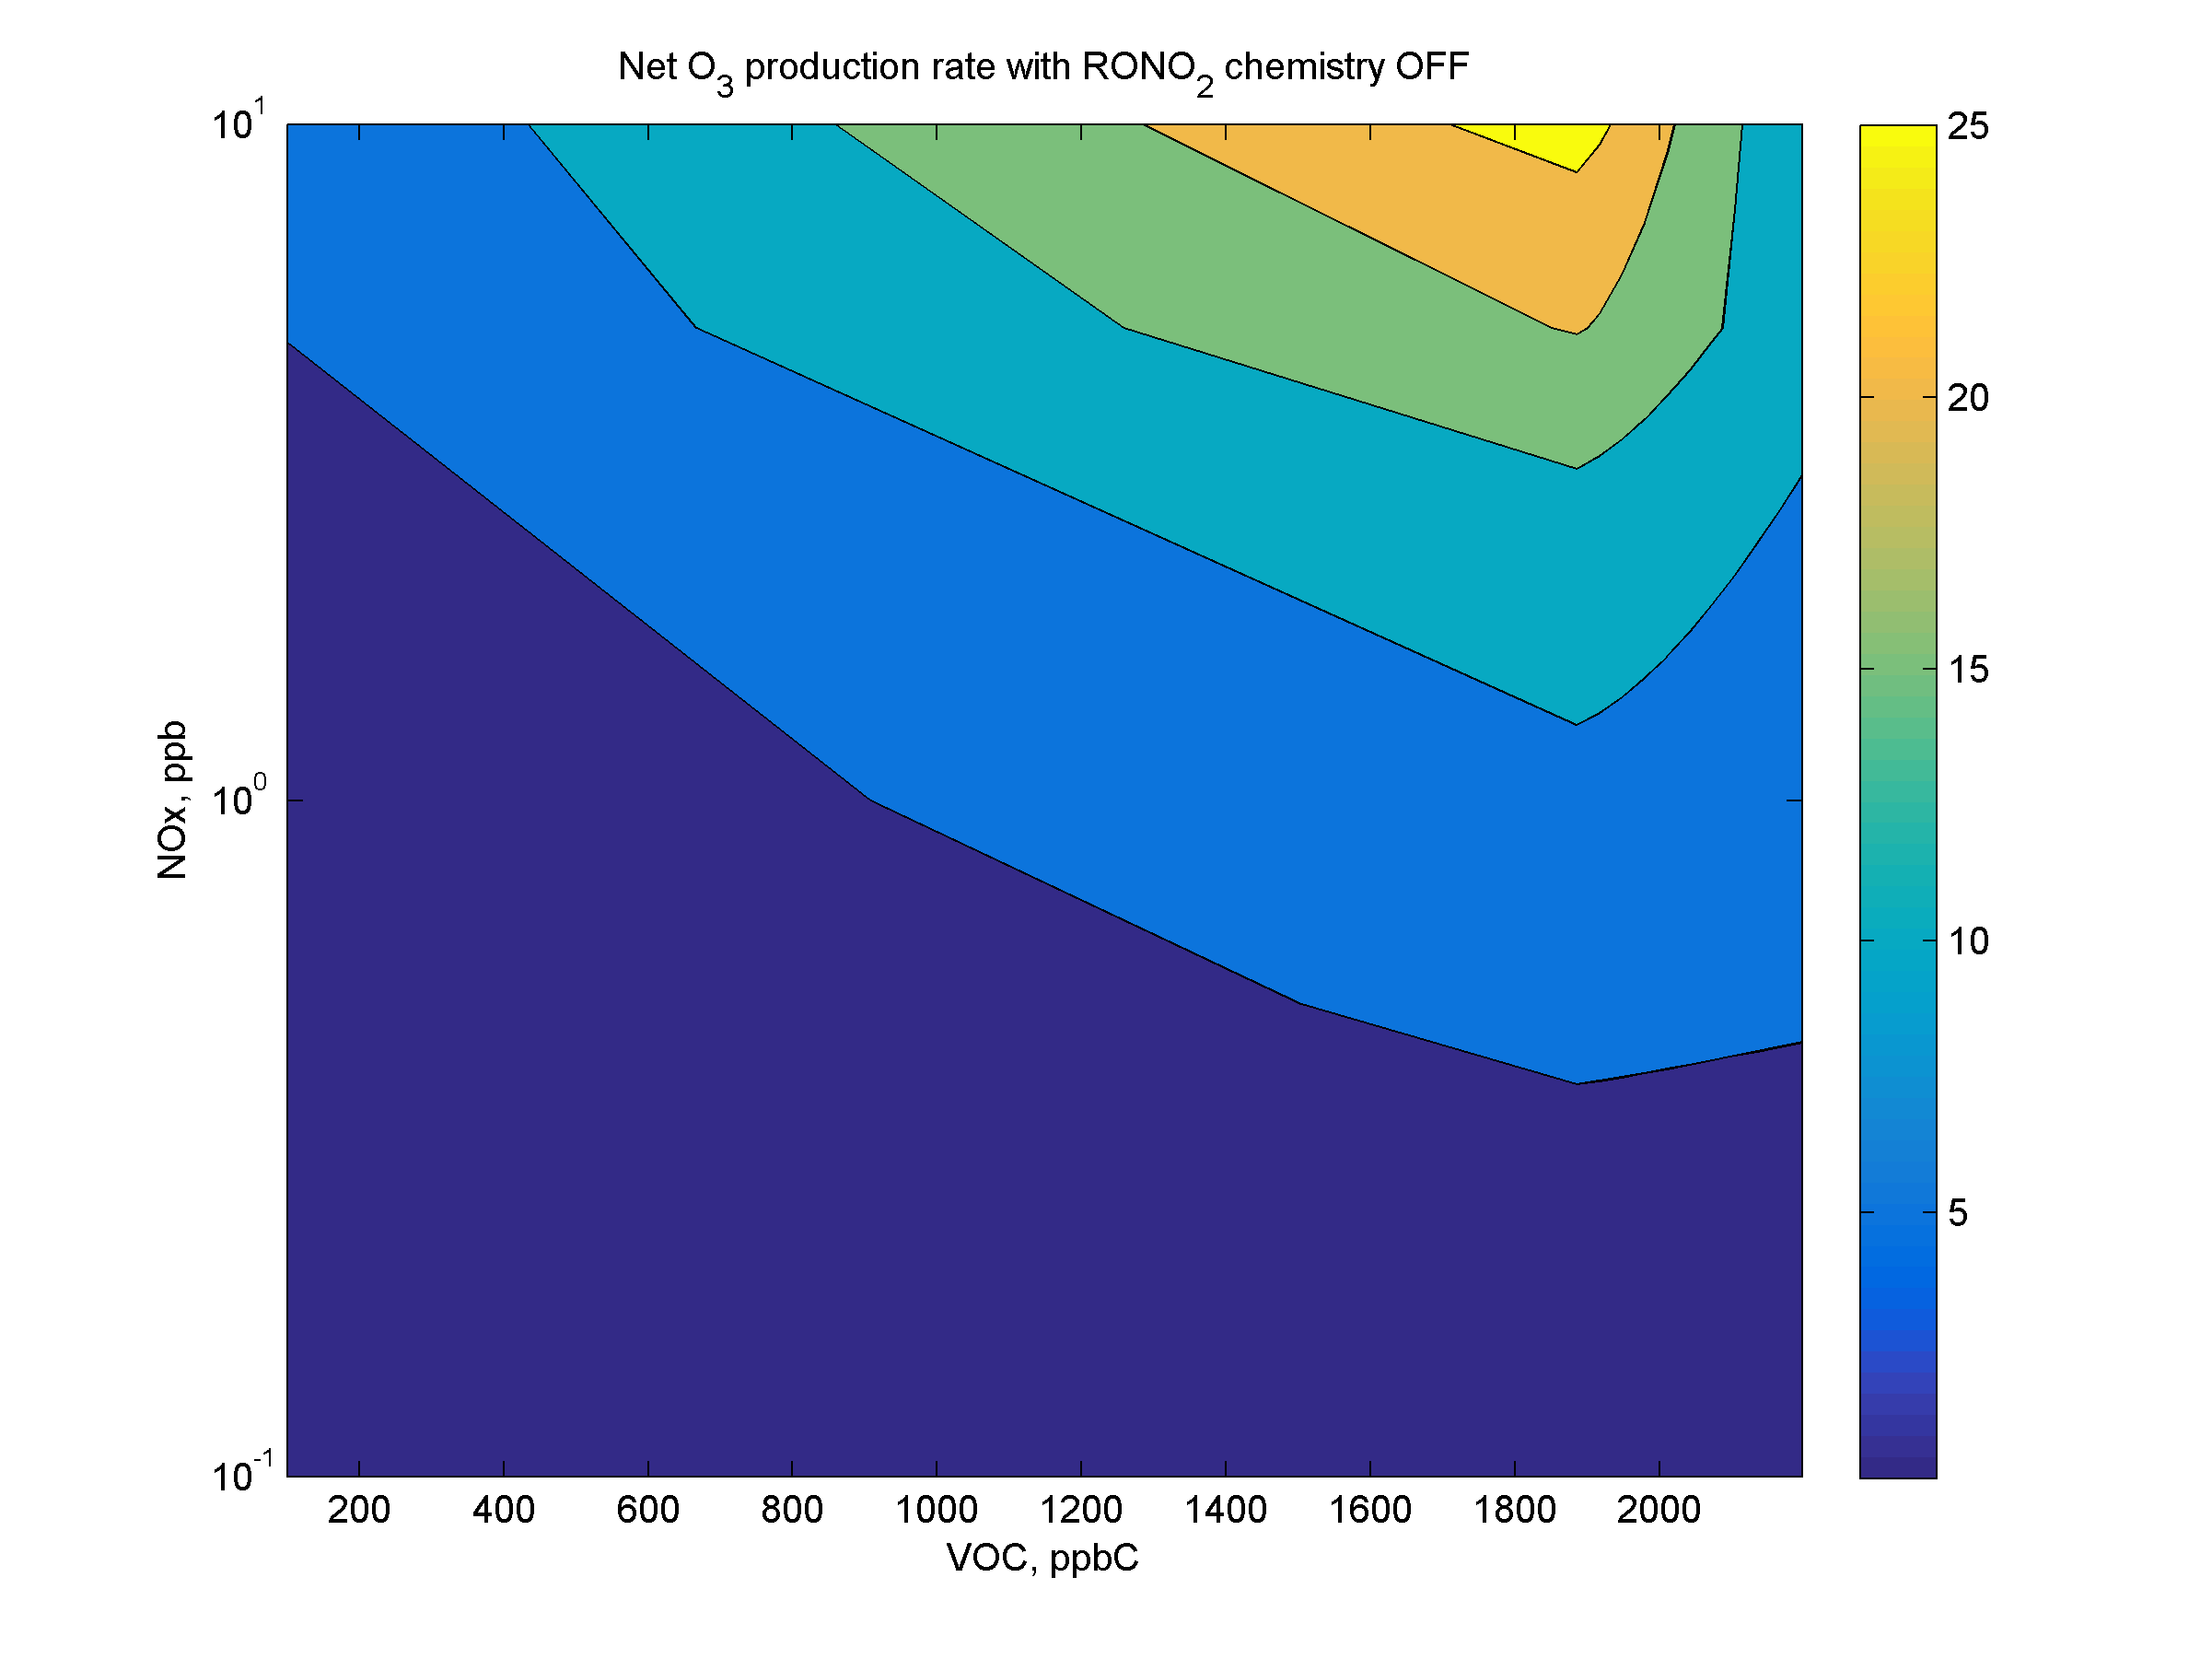
\includegraphics[width=.99\linewidth]{D:/FACSIMILE/ANsCBmodel/matlab/ANsCB_pics/ANsNOxVOC/noAN/chem_noAN_netO3rate_withINORG_NOx_1ppb_100ppb.png}
  \captionof{figure}{Isopleths giving net rate of $O_3$ production (ppb/h, color) as a function of $VOC$ (ppbC) and $NO_x$ (ppb) in the first modelling experiment with alkyl nitrate chemistry switched off combined with an additional run with inorganic chemistry only (i.e. the only $VOC$ is $CO$).}\label{fig:noAN_netO3rate}
\end{minipage}
\end{figure}

Rewrite!

The same kind of plot can be found in Figure \ref{fig:noAN_netO3rate}, which is produced using data from our model from the first experiment with alkyl nitrate chemistry switched off. Taking into account the fact that the maximum $NO_x$ mixing ratio considered in the experiment is 10 ppb, our results are directly comparable only with a part of the data from Figure \ref{fig:Sillman1999}, namely with those inside the green dashed square. Moreover, since the minimum $NO_x$ mixing ratio considered in the experiment is 5 ppt, while the corresponding value in Figure \ref{fig:Sillman1999} is 1 ppb, a negative $O_3$ production rate is seen in our results, whereas it stays out of range of Figure \ref{fig:Sillman1999}.

One can see the same pattern in these two figures. At high $VOC$/$NO_x$ ratios, the rate of $O_3$ production increases with increasing $NO_x$ and reaches its maximum at the highest $NO_x$ and $VOC$ levels (which corresponds to the top right corner of the green dashed square). The change in $O_3$ production rate at high $VOC$/$NO_x$ ratios in our model is largely insensitive to $VOC$, which fits into the theory. At low $VOC$/$NO_x$ ratios the $O_3$ production rate starts to depend on $VOC$ concentration also resembling the behaviour of ozone isopleths at the top left corner of the green dashed square. The overall tendency of $O_3$ production rate to increase with increasing $VOC$ and $NO_x$ is present in both figures showing that the model reproduces this feature according to the theory. However, the modelled values of $O_3$ production rates are much lower than those in Figure \ref{fig:Sillman1999}: in the model the maximum production rate is 9 ppb/h, while in theory it is 30 ppb/h, meaning that our model underestimates the $O_3$ production rate, but reproduces some features of the relationship between $O_3$, $NO_x$ and $VOC$.

\section{Results} \label{sec:res}
\subsection{Sensitivity of $O_3$ production to alkyl nitrate chemistry}

A number of simulations for evaluating the sensitivity of the $O_3$ production to alkyl nitrate chemistry were carried out. This was accomplished by switching on and off all reactions present in the chemical mechanism that describe formation or destruction of all alkyl nitrates.

\begin{figure}
\centering
\begin{minipage}{.3\textwidth}
  \centering
  \includegraphics[width=.99\linewidth]{D:/FACSIMILE/ANsCBmodel/matlab/ANsCB_pics/ANsNOxVOC/noAN/chem_noAN_netO3rate_noINORG_NOx_5ppt_100ppb.png}
\end{minipage}
\begin{minipage}{.3\textwidth}
  \centering
  \includegraphics[width=.99\linewidth]{D:/FACSIMILE/ANsCBmodel/matlab/ANsCB_pics/ANsNOxVOC/allAN/chem_allAN_netO3rate_noINORG_NOx_5ppt_100ppb.png}
\end{minipage}
\begin{minipage}{.3\textwidth}
  \centering
  \includegraphics[width=.99\linewidth]{D:/FACSIMILE/ANsCBmodel/matlab/ANsCB_pics/ANsNOxVOC/allAN/chem_allAN_netO3ratediff_noINORG_NOx_5ppt_100ppb.png}
\end{minipage}
\caption{Isopleths giving net rate of $O_3$ production (ppb/h, color) as a function of $VOC$ (ppbC) and $NO_x$ (ppb) with alkyl nitrate chemistry switched off (left) and switched on (middle). Difference between them is shown on the right.}
\end{figure}

The simulations that compared ... provided insight into which reactions... under changing $NO_x$ mixing ratios (Table ...).

%\begin{figure}[h] % allAN_netO3_rate
%\includegraphics[width=\linewidth]{D:/FACSIMILE/ANsCBmodel/matlab/ANsCB_pics/ANsNOxVOC/allAN/chem_allAN_netO3_rate.png}
%\caption{allAN, netO3 rate}\label{fig:allAN_netO3_rate}
%\end{figure}

! Dependence of alkyl nitrate yield on carbon number (paper about n-alkanes): bigger yield of ANs from larger carbon number means that the potential for contributing to photochemical air pollution may be less for the larger (C>6) n-alkanes that for the smaller ones.

\section{Discussion} \label{sec:discuss}
The experimental results presented in the previous section provide an opportunity to speculate about the behaviour of our simple model of alkyl nitrate production and loss with time in comparison with the observational data. 

\section{Conclusion} \label{sec:conclusion}
\bibliography{diss_refs}

\section{Appendix I} \label{sec:appendix1}

\end{document}
